\subsection{Zustandshaltung der Pipeline}

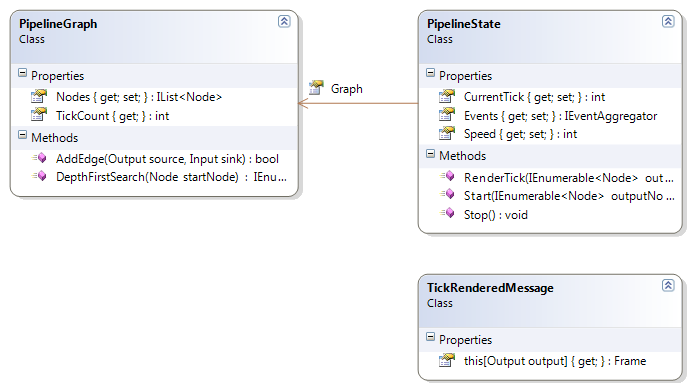
\includegraphics[width=\textwidth]{YuvKA.Pipeline/states.png}
Diese Gruppe von Klassen dient dazu, den Zustand der Pipeline zu verwalten. Der \name{PipelineState} benutzt zur Verwaltung der im Pipeline-Graphen vorhandenen Knoten und Kanten den \name{PipelineGraph}. Er ist zudem dafür zuständig, die Berechnung der Pipeline zu starten und zu stoppen. Die \name{TickRenderedMessage} wird geworfen, wenn ein Zeitabschnitt berechnet ist.

\subsubsection{YuvKA.Pipeline.PipelineState}

\begin{verbatim}
[DataContract]
public class PipelineState
\end{verbatim}

\paragraph{Beschreibung}~\\
Die Klasse \name{PipelineState} vereint in sich den Gesamtzustand des Datenmodells, womit durch ihre Serialisierung alle relevanten Programmdaten gespeichert werden. Sie enthält den aktuellen Wiedergabestatus und bietet zur Wiedergabe eine Schnittstelle zum \name{PipelineDriver}.

\paragraph{Typmember}
\begin{itemize}

\property{CurrentTick}
	\begin{verbatim}
	[DataMember]
	public int CurrentTick { get; set; }
	\end{verbatim} 
	Ruft den als nächstes zu berechnenden Tick ab oder legt ihn fest. Das Neusetzen der Property führt zum Abbruch der Berechnung des aktuellen Ticks.

\property{Speed}
	\begin{verbatim}
	[DataMember]
	public int Speed { get; set; }
	\end{verbatim}
	Ruft die Abspielgeschwindigkeit in Frames pro Sekunde ab oder legt sie fest.

\property{Graph}
	\begin{verbatim}
	[DataMember]
	public PipelineGraph Graph { get; }
	\end{verbatim}
	Ruft den \name{PipelineGraph} ab, welcher die Struktur der Pipeline repräsentiert.

\property{Events}
	\begin{verbatim}
	[Import(typeof(IEventAggregator))]
	public IEventAggregator Events { get; set; }
	\end{verbatim}
	Per Dependency Injection injizierte Schnittstelle zum Caliburn Message System, über das die Ausgabefenster über die Beendigung aller im aktuellen Tick berechneten \name{Frame}s benachrichtigt werden.

\method{Start}
	\begin{verbatim}
	public void Start(IEnumerable<Node> outputNodes)
	\end{verbatim}
	Weist den \name{PipelineDriver} an, die Pipeline ab dem aktuellen Tick für die gegebenen Knoten zu berechnen. Pro abgeschlossener Berechnung eines Ticks wird eine \name{TickRenderedMessage} geworfen.

\method{Stop}
	\begin{verbatim}
	public void Stop()
	\end{verbatim}
	Beendet die Wiedergabe und stoppt den \name{PipelineDriver}. Danach vom \name{PipelineDriver} asynchron erhaltene \name{Frame}s werden ignoriert.

\method{Stop}
	\begin{verbatim}
	public void RenderTick(IEnumerable<Node> outputNodes)
	\end{verbatim}
	Weist den \name{PipelineDriver} an, die Pipeline für den aktuellen Tick und die gegebenen Knoten zu berechnen. Bei abgeschlossener Berechnung wird eine \name{TickRenderedMessage} geworfen.
\end{itemize}

\subsubsection{YuvKA.Pipeline.PipelineGraph}
	
\begin{verbatim}
[DataContract]
public class PipelineGraph	
\end{verbatim}

\paragraph{Beschreibung}~\\
Die Klasse \name{PipelineGraph} verwaltet den Aufbau des Pipeline-Graphen. 
	
\paragraph{Typmember}
\begin{itemize}

\property{Nodes}
	\begin{verbatim}
	[DataMember]
	public IList<Node> Nodes { get; }
	\end{verbatim}
	Verwaltet die im Pipeline-Graphen verfügbaren Knoten und ruft sie ab.

\property{FrameCount}
	\begin{verbatim}
	[DataMember]
	public int FrameCount { get; }
	\end{verbatim}
	Ruft die maximale Länge aller als Input gegebenen Videos ab.


	
\method{AddEdge}
	\begin{verbatim}
	public bool AddEdge(Output source, Input sink)
	\end{verbatim}
	Wenn die durch \name{source} und \name{sink} spezifizierte Kante zu keinem Zyklus innerhalb des Pipeline-Graphen führt, so soll sie durch Setzen der Source-Property von \name{sink} als \name{source} hinzugefügt und true ausgegeben werden. Andernfalls soll die Kante nicht zum Graphen hinzugefügt und false ausgegeben werden.

\method{DepthFirstSearch}
    \begin{verbatim}
    public IEnumerable<Node> DepthFirstSearch(Node startNode)
    \end{verbatim}
    Führt eine Tiefensuche auf dem Graphen aus und liefert eine Liste gefundener Knoten in topologischer Reihenfolge zurück. Dies wird für die Zyklensuche im Graph benötigt.

\end{itemize}
	
\subsubsection{YuvKA.Pipeline.TickRenderedMessage}
		
\begin{verbatim}
public class TickRenderedMessage
\end{verbatim}

\paragraph{Beschreibung}~\\
Die Klasse \name{TickRenderedMessage} enthält die im letzten Tick berechneten \name{Frame}s aller \name{Output}s.

\paragraph{Typmember}
\begin{itemize}
	
\property{this[]}
	\begin{verbatim}
	public Frame this[Output output] { get; }
	\end{verbatim}
Indexer. Ruft den durch \name{output} spezifizierten \name{Frame} auf.

\end{itemize}
